\documentclass{beamer}
 
\usepackage[utf8]{inputenc}
\usepackage{geometry}
\usepackage{amsmath}
\usepackage{amsthm}
\usepackage{amssymb}
\usepackage{graphicx}
\usepackage{subfigure}
\usepackage{tikz}
\usepackage{url}
\usepackage{dirtytalk}

\usetheme{Madrid}
\usecolortheme{default}
 
\usetikzlibrary{patterns}

\def\hexagonsize{0.2cm}
\pgfdeclarepatternformonly
  {hexagons}% name
  {\pgfpointorigin}% lower left
  {\pgfpoint{3*\hexagonsize}{0.866025*2*\hexagonsize}}%  upper right
  {\pgfpoint{3*\hexagonsize}{0.866025*2*\hexagonsize}}%  tile size
  {% shape description
   \pgfsetlinewidth{1.2pt}
   \pgftransformshift{\pgfpoint{0mm}{0.866025*\hexagonsize}}
   \pgfpathmoveto{\pgfpoint{0mm}{0mm}}
   \pgfpathlineto{\pgfpoint{0.5*\hexagonsize}{0mm}}
   \pgfpathlineto{\pgfpoint{\hexagonsize}{-0.866025*\hexagonsize}}
   \pgfpathlineto{\pgfpoint{2*\hexagonsize}{-0.866025*\hexagonsize}}
   \pgfpathlineto{\pgfpoint{2.5*\hexagonsize}{0mm}}
   \pgfpathlineto{\pgfpoint{3*\hexagonsize+0.2mm}{0mm}}
   \pgfpathmoveto{\pgfpoint{0.5*\hexagonsize}{0mm}}
   \pgfpathlineto{\pgfpoint{\hexagonsize}{0.866025*\hexagonsize}}
   \pgfpathlineto{\pgfpoint{2*\hexagonsize}{0.866025*\hexagonsize}}
   \pgfpathlineto{\pgfpoint{2.5*\hexagonsize}{0mm}}
   \pgfusepath{stroke}
  } 

\newcommand{\Tube}[6][]%
% [further options], width, iterations, inner color, outer color, path definition
{   \colorlet{InColor}{#4}
    \colorlet{OutColor}{#5}
    \foreach \I in {1,...,#3}
    {   \pgfmathsetlengthmacro{\h}{(\I-1)/#3*#2}
        \pgfmathsetlengthmacro{\r}{sqrt(pow(#2,2)-pow(\h,2))}
        \pgfmathsetmacro{\c}{(\I-0.5)/#3*100}
        \draw[InColor!\c!OutColor, line width=\r, #1] #6;
    } 
} %draws a 3D-tube, see https://tex.stackexchange.com/questions/148379/define-a-path-like-command-in-tikz-to-draw-3d-tubes for details

%Commands for mathematical symbols that we frequently use
\newcommand{\reals}{\mathbb{R}}
\newcommand{\compx}{\mathbb{C}}
\newcommand{\rationals}{\mathbb{Q}}
\newcommand{\integers}{\mathbb{Z}}
\newcommand{\naturals}{\mathbb{N}}
\newcommand{\graph}{\mathbb{G}}
\newcommand{\ceil}[1]{\left\lceil #1 \right\rceil}

%Commands for maths formatting; grads, fractions, etc
\newcommand{\abs}[1]{\lvert #1 \rvert}
\newcommand{\recip}[1]{\frac{1}{#1}}
\newcommand{\half}{\recip{2}}
\newcommand{\grad}{\nabla}
\newcommand{\laplacian}{\nabla^{2}}
\newcommand{\bracs}[1]{\left( #1 \right)}
\newcommand{\sqbracs}[1]{\left[ #1 \right]}
\newcommand{\diff}[1]{\dfrac{\mathrm{d}}{\mathrm{d}#1}}
\newcommand{\pdiff}[1]{\dfrac{\partial}{\partial #1}}
\newcommand{\ddiff}[1]{\dfrac{\mathrm{d}^{2}}{\mathrm{d}^{2}#1}}
\renewcommand{\epsilon}{\varepsilon} %i want nice epsilons
\newcommand{\set}[1]{\left\{ #1 \right\}}
\newcommand{\vU}{\mathbf{U}} %vectorised U
\newcommand{\vx}{\mathbf{x}} %vector x
\newcommand{\vy}{\mathbf{y}} %vector y
\newcommand{\eval}[1]{\Big|_{#1}}
\newcommand{\lp}[2]{L^{#1}\bracs{#2}}
\newcommand{\Hp}[2]{H^{#1}\bracs{#2}}
\newcommand{\mathset}[1]{\left\{ #1 \right\}}
\newcommand{\norm}[1]{\left\vert\left\vert #1 \right\vert\right\vert}

%Variable names etc, change macro rather than every symbol!
\newcommand{\trfn}{\Xi} %the symbol for the transcendental analysis involving omega
\newcommand{\homDomain}{\Omega} %whatever symbol I want to use for the homogenisation problem's domain
\newcommand{\perBoundary}{\Gamma_{\mathrm{p}}}
\newcommand{\othBoundary}{\Gamma_{0}}
\newcommand{\femSolSpace}{H^{1}\bracs{\homDomain}} %for the solution space of u
\newcommand{\rInd}[1]{N_{\mathrm{#1}}}
\newcommand{\ang}[1]{\theta_{\mathrm{#1}}}
\newcommand{\eVol}{V^{\mathrm{(E)}}}
\newcommand{\vVol}{V^{\mathrm{(V)}}} %vertex and edge volumes
\newcommand{\graphOp}{\mathcal{A}} %operator on graphs
\newcommand{\nodeSet}{\mathcal{N}} %node set for FEM
\newcommand{\eleSet}{\mathcal{T}} %element set for FEM
\newcommand{\magP}{\mu} %magnetic permeability
\newcommand{\elcP}{\epsilon_{\mathrm{p}}} %electric permitivitty
\newcommand{\tho}{\theta_{1}}
\newcommand{\tht}{\theta_{2}}
 
%removes figure prefix from captions
\setbeamertemplate{caption}{\raggedright\insertcaption\par} 
 
%Information to be included in the title page
\title{Asymptotic and Numerical Analysis of Wave Propagation in Photonic Fibres with a Thin-Structure Cladding.}
\author{William Graham}
\institute{University of Bath}
\date{\today}
 
\begin{document}
 
\frame{\titlepage}
 
%slide on my pre-samba background and project details
\begin{frame}
	\frametitle{My Background}

	\begin{block}{Undergraduate}
		MSci Maths \& Physics, University of Bath (Dept. of Physics)
	\end{block}
	
	\begin{block}{At SAMBa}
	Supervisors
		\begin{itemize}
			\item Dr Kirill Cherednichenko (Maths)
			\item Prof David Bird (Physics)
		\end{itemize}
	PhD Project Title
		\begin{itemize}
			\item Asymptotic and Numerical Analysis of Wave Propagation in Photonic Fibres with a Thin-Structure Cladding
		\end{itemize}
	\end{block}

\end{frame} 

%slide on the motivation for my research
\begin{frame}
	\frametitle{Project Motivation}
	
	Photonic Crystal Fibres 
	\begin{itemize}
		\item A (relatively) new design of optical fibre \cite{knight2003photonic}
	\end{itemize}
	
	\begin{figure}
		\centering
		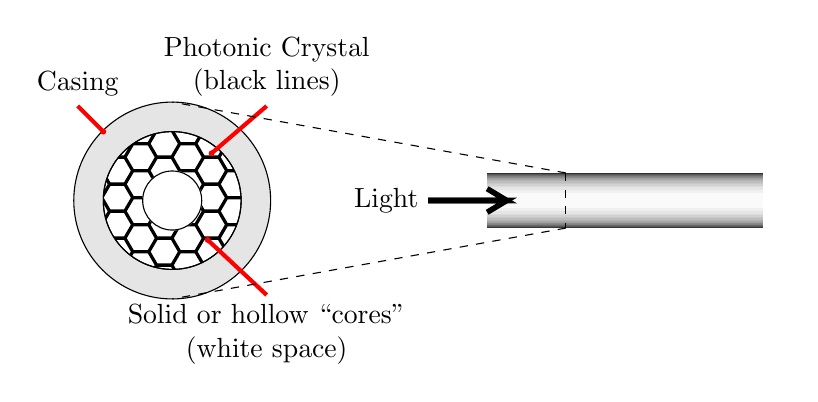
\begin{tikzpicture}
			\begin{scope}[scale=0.5]
				\filldraw[fill=black!10!white, draw=black] (0,0) circle (2.5);
				\draw[line width=1.5, color=red] (-1.75,1.75) -- (-2.4,2.4);
				\node[anchor=south] at (-2.4,2.4) {Casing};
				\fill[color=red] (-1.75,1.75) circle (0.075); %casing and label
				\filldraw[fill=white, draw=black] (0,0) circle (1.75);
				\filldraw[pattern=hexagons, draw=black] (0,0) circle (1.75); %hexagons
				\draw[line width=1.5, color=red] (1.0,1.2) -- (2.4,2.4);
				\fill[color=red] (1.0, 1.2) circle (0.075);
				\node[anchor=south, align=center] at (2.4,2.4) {Photonic Crystal \\ (black lines)};
				\node[anchor=north, align=center] at (2.4,-2.4) {Solid or hollow \say{cores} \\ (white space)};
				\draw[line width=1.5, color=red] (0.9,-1.0) -- (2.4,-2.4);
				\fill[color=red] (0.9, -1.0) circle (0.075);
				%core circle
				\filldraw[color=white] (0,0) circle (0.75);
				\draw[color=black] (0,0) circle (0.75);
				
				%tube part
				\Tube{7mm}{25}{white}{black}{(8,0) to[out=0,in=180] (15,0)};
				\draw[dashed] (10,-0.7) -- (0,-2.5);
				\draw[dashed] (10,0.7) -- (0,2.5);
				\draw[dashed] (10,0.7) -- (10,-0.7);
				\draw[line width=2] (6.5,0) -- (8.5,0) -- (8,0.3);
				\draw[line width=2] (6.5,0) -- (8.5,0) -- (8,-0.3);
				\node[anchor=east, align=center] at (6.5,0) {Light};
			\end{scope}
		\end{tikzpicture}
	\end{figure}
	
	Usable light frequencies highly dependant on geometry and material.	
	
\end{frame}

%slide on what I'm actually doing right now
\begin{frame}
	\frametitle{My Research}
	
	\begin{block}{In One Sentence}
		``Studying features of Maxwell problems on fibre-like geometries"
	\end{block}
	
	\begin{block}{The Broader Context}
		\begin{itemize}
			\item Mathematical treatment of \textit{thin-structure} and \textit{singular structure} geometries \cite{zhikov2000extension}
			\item Understanding the link between geometry and spectra \cite{exner2005convergence}
			\item In-depth analysis of physically interesting systems \cite{cooper2014bandgaps}
		\end{itemize}
	\end{block}
	
	\begin{block}{How?}
		\begin{itemize}
			\item Homogenization theory
			\item Technical/rigorous  problem formulation
			\item Numerical experiments
		\end{itemize}
	\end{block}
	
\end{frame}

%slide for references
\begin{frame}
	\frametitle{References}
	
	\bibliographystyle{unsrt}
	\bibliography{../TFR/Latex/TFRBib.bib}
\end{frame}
 
\end{document}
